\documentclass[12pt, titlepage]{article}

\usepackage{fullpage}
\usepackage[round]{natbib}
\usepackage{multirow}
\usepackage{booktabs}
\usepackage{tabularx}
\usepackage{graphicx}
\usepackage{float}
\usepackage{hyperref}
\hypersetup{
    colorlinks,
    citecolor=blue,
    filecolor=black,
    linkcolor=red,
    urlcolor=blue
}

%% Comments

\usepackage{color}

\newif\ifcomments\commentstrue %displays comments
%\newif\ifcomments\commentsfalse %so that comments do not display

\ifcomments
\newcommand{\authornote}[3]{\textcolor{#1}{[#3 ---#2]}}
\newcommand{\todo}[1]{\textcolor{red}{[TODO: #1]}}
\else
\newcommand{\authornote}[3]{}
\newcommand{\todo}[1]{}
\fi

\newcommand{\wss}[1]{\authornote{blue}{SS}{#1}} 
\newcommand{\plt}[1]{\authornote{magenta}{TPLT}{#1}} %For explanation of the template
\newcommand{\an}[1]{\authornote{cyan}{Author}{#1}}

%% Common Parts

\newcommand{\progname}{Software Eng} % PUT YOUR PROGRAM NAME HERE
\newcommand{\authname}{Team \#, Team Name
\\ Student 1 Matthew Collard
\\ Student 2 Sam Gorman
\\ Student 3 Ethan Kannampuzha
\\ Student 4 Kieran Gara} % AUTHOR NAMES                  

\usepackage{hyperref}
    \hypersetup{colorlinks=true, linkcolor=blue, citecolor=blue, filecolor=blue,
                urlcolor=blue, unicode=false}
    \urlstyle{same}
                                


\newcounter{acnum}
\newcommand{\actheacnum}{AC\theacnum}
\newcommand{\acref}[1]{AC\ref{#1}}

\newcounter{ucnum}
\newcommand{\uctheucnum}{UC\theucnum}
\newcommand{\uref}[1]{UC\ref{#1}}

\newcounter{mnum}
\newcommand{\mthemnum}{M\themnum}
\newcommand{\mref}[1]{M\ref{#1}}

\begin{document}

\title{Module Guide for \progname{}} 
\author{\authname}
\date{\today}

\maketitle

\pagenumbering{roman}

\section{Revision History}

\begin{tabularx}{\textwidth}{p{3cm}p{2cm}X}
\toprule {\bf Date} & {\bf Version} & {\bf Notes}\\
\midrule
January 13, 2024 & 1.0 & Initial changes \\
January 14 & 1.1 & Module hierarchy chart and specifications\\
January 17 & 1.2 & Revision 0\\
\bottomrule
\end{tabularx}

\newpage

\section{Reference Material}

This section records information for easy reference.

\subsection{Abbreviations and Acronyms}

\renewcommand{\arraystretch}{1.2}
\begin{tabular}{l l} 
  \toprule		
  \textbf{symbol} & \textbf{description}\\
  \midrule 
  
  AC & Anticipated Change\\
  AR & Augmented Reality\\
  DAG & Directed Acyclic Graph \\
  M & Module \\
  MG & Module Guide \\
  OS & Operating System \\
  R & Requirement\\
  SC & Scientific Computing \\
  SRS & Software Requirements Specification\\
  \progname & Explanation of program name\\
  UC & Unlikely Change \\
  \wss{etc.} & \wss{...}\\
  \bottomrule
\end{tabular}\\

\newpage

\tableofcontents

\listoftables

\listoffigures

\newpage

\pagenumbering{arabic}

\section{Introduction}

Decomposing a system into modules is a commonly accepted approach to developing
software.  A module is a work assignment for a programmer or programming
team~\citep{ParnasEtAl1984}.  We advocate a decomposition
based on the principle of information hiding~\citep{Parnas1972a}.  This
principle supports design for change, because the ``secrets'' that each module
hides represent likely future changes.  Design for change is valuable in SC,
where modifications are frequent, especially during initial development as the
solution space is explored.  

Our design follows the rules layed out by \citet{ParnasEtAl1984}, as follows:
\begin{itemize}
\item System details that are likely to change independently should be the
  secrets of separate modules.
\item Each data structure is implemented in only one module.
\item Any other program that requires information stored in a module's data
  structures must obtain it by calling access programs belonging to that module.
\end{itemize}

After completing the first stage of the design, the \href{https://github.com/SammyG7/Mac-AR/blob/main/docs/SRS/SRS.pdf}{System Requirement Specifications} (SRS), the Module Guide (MG) is developed~\citep{ParnasEtAl1984}. The MG
specifies the modular structure of the system and is intended to allow both
designers and maintainers to easily identify the parts of the software.  The
potential readers of this document are as follows:

\begin{itemize}
\item New project members: This document can be a guide for a new project member
  to easily understand the overall structure and quickly find the
  relevant modules they are searching for.
\item Maintainers: The hierarchical structure of the module guide improves the
  maintainers' understanding when they need to make changes to the system. It is
  important for a maintainer to update the relevant sections of the document
  after changes have been made.
\item Designers: Once the module guide has been written, it can be used to
  check for consistency, feasibility, and flexibility. Designers can verify the
  system in various ways, such as consistency among modules, feasibility of the
  decomposition, and flexibility of the design.
\end{itemize}

The rest of the document is organized as follows. Section
\ref{SecChange} lists the anticipated and unlikely changes of the software
requirements. Section \ref{SecMH} summarizes the module decomposition that
was constructed according to the likely changes. Section \ref{SecConnection}
specifies the connections between the software requirements and the
modules. Section \ref{SecMD} gives a detailed description of the
modules. Section \ref{SecTM} includes two traceability matrices. One checks
the completeness of the design against the requirements provided in the SRS. The
other shows the relation between anticipated changes and the modules. Section
\ref{SecUse} describes the use relation between modules.

\section{Anticipated and Unlikely Changes} \label{SecChange}

This section lists possible changes to the system. According to the likeliness
of the change, the possible changes are classified into two
categories. Anticipated changes are listed in Section \ref{SecAchange}, and
unlikely changes are listed in Section \ref{SecUchange}.

\subsection{Anticipated Changes} \label{SecAchange}

Anticipated changes are the source of the information that is to be hidden
inside the modules. Ideally, changing one of the anticipated changes will only
require changing the one module that hides the associated decision. The approach
adapted here is called design for
change.

\begin{description}
\item[\refstepcounter{acnum} \actheacnum \label{acInput2}:] Additional puzzle modules
\item[\refstepcounter{acnum} \actheacnum \label{acInput3}:] Modification of puzzles to allow to involve more users
\item[\refstepcounter{acnum} \actheacnum \label{acInput4}:] Update library versions used in the creation of the application (such as Vivox)
\item[\refstepcounter{acnum} \actheacnum \label{acInput5}:] The user interface layout of the application
\item[\refstepcounter{acnum} \actheacnum \label{acInput6}:] The number of users that can use the application at one time (database/network size)
\item[\refstepcounter{acnum} \actheacnum \label{acInput7}:] The number of users that can play cooperatively in the same game room
\end{description}

\subsection{Unlikely Changes} \label{SecUchange}

The module design should be as general as possible. However, a general system is
more complex. Sometimes this complexity is not necessary. Fixing some design
decisions at the system architecture stage can simplify the software design. If
these decision should later need to be changed, then many parts of the design
will potentially need to be modified. Hence, it is not intended that these
decisions will be changed.

\begin{description}
\item[\refstepcounter{ucnum} \uctheucnum \label{ucIO}:] The engine that the application is made from (ie. Unity engine)
\item[\refstepcounter{ucnum} \uctheucnum \label{ucIO}:] The addition of an account system for users
\item[\refstepcounter{ucnum} \uctheucnum \label{ucIO}:] The ability to play non-cooperatively (single player)
\item[\refstepcounter{ucnum} \uctheucnum \label{ucIO}:] The environment that the user will access the game environment from
\item[\refstepcounter{ucnum} \uctheucnum \label{ucIO}:] User input for gameplay controls
\end{description}

\section{Module Hierarchy} \label{SecMH}

This section provides an overview of the module design. Modules are summarized
in a hierarchy decomposed by secrets in Table \ref{TblMH}. The modules listed
below, which are leaves in the hierarchy tree, are the modules that will
actually be implemented.

\begin{description}
%\item [\refstepcounter{mnum} \mthemnum \label{mHH}:] Hardware-Hiding Module
\item [\refstepcounter{mnum} \mthemnum \label{mHardware}:] Hardware Module

\item [\refstepcounter{mnum} \mthemnum \label{mGameRoom}:] Game Room Module
\item [\refstepcounter{mnum} \mthemnum \label{mText}:] Text Communication Module
\item [\refstepcounter{mnum} \mthemnum \label{mVoice}:] Voice Communication Module
\item [\refstepcounter{mnum} \mthemnum \label{mGameSave}:] Game Save Module
\item [\refstepcounter{mnum} \mthemnum \label{mMultiplayerPuzzle}:] Multiplayer Puzzle Module

\item 
[\refstepcounter{mnum} \mthemnum \label{mPSimon}:] Simon Says Puzzle Module
\item 
[\refstepcounter{mnum} \mthemnum \label{mPCode}:] Code Puzzle Module
\item 
[\refstepcounter{mnum} \mthemnum \label{mPWires}:] Wires Puzzle Module
\item 
[\refstepcounter{mnum} \mthemnum \label{mPMaze}:] Maze Puzzle Module
\item 
[\refstepcounter{mnum} \mthemnum \label{mPMath}:] Math Puzzle Module
\item 
[\refstepcounter{mnum} \mthemnum \label{mPBomb}:] Bomb Puzzle Module
\item [\refstepcounter{mnum} \mthemnum \label{mDatabase}:] Database/Network Manager Module
\item [\refstepcounter{mnum} \mthemnum \label{mErrorManager}:] Error Manager Module
\item [\refstepcounter{mnum} \mthemnum \label{mDoc}:] Documentation Module
\end{description}


\begin{table}[h!]
\centering
\begin{tabular}{p{0.3\textwidth} p{0.6\textwidth}}
\toprule
\textbf{Level 1} & \textbf{Level 2}\\
\midrule

{Hardware-Hiding Module} & Hardware Module \\
\midrule

\multirow{7}{0.3\textwidth}{Behaviour-Hiding Module}
& Game Room Module\\
& Text Communication Module\\
& Voice Communication Module\\
& Game Save Module\\
& Multiplayer Puzzle Module\\
& Simon Says Puzzle Module\\
& Code Puzzle Module\\
& Wires Puzzle Module\\
& Maze Puzzle Module\\
& Math Puzzle Module\\
& Bomb Puzzle Module\\
\midrule

\multirow{3}{0.3\textwidth}{Software Decision Module} & Database/Network Manager Module\\
& Error Manager Module\\
& Documentation Module\\
\bottomrule

\end{tabular}
\caption{Module Hierarchy}
\label{TblMH}
\end{table}

\newpage
\section{Connection Between Requirements and Design} \label{SecConnection}

The design of the system is intended to satisfy the requirements developed in
the SRS. In this stage, the system is decomposed into modules. The connection
between requirements and modules is listed in Table~\ref{TblRT}.

\section{Module Decomposition} \label{SecMD}

Modules are decomposed according to the principle of ``information hiding''
proposed by \citet{ParnasEtAl1984}. The \emph{Secrets} field in a module
decomposition is a brief statement of the design decision hidden by the
module. The \emph{Services} field specifies \emph{what} the module will do
without documenting \emph{how} to do it. For each module, a suggestion for the
implementing software is given under the \emph{Implemented By} title. If the
entry is \emph{OS}, this means that the module is provided by the operating
system or by standard programming language libraries.  \emph{\progname{}} means the
module will be implemented by the \progname{} software.

Only the leaf modules in the hierarchy have to be implemented. If a dash
(\emph{--}) is shown, this means that the module is not a leaf and will not have
to be implemented.

\subsection{Hardware Hiding Module (\mref{mHardware})}

\begin{description}
\item[Secrets:]The data structure and algorithm used to implement the virtual
  hardware.
\item[Services:]Serves as a virtual hardware used by the rest of the
  system. This module provides the interface between the hardware and the
  software. So, the system can use it to display outputs or to accept inputs.
\item[Implemented By:] OS
\end{description}

\subsection{Behaviour-Hiding Module}

\begin{description}
\item[Secrets:]The contents of the required behaviours.
\item[Services:]Includes programs that provide externally visible behaviour of
  the system as specified in the software requirements specification (SRS)
  documents. This module serves as a communication layer between the
  hardware-hiding module and the software decision module. The programs in this
  module will need to change if there are changes in the SRS.
\item[Implemented By:] Mac-AR
\end{description}

\subsubsection{Game Room Module (\mref{mGameRoom})}

\begin{description}
\item[Secrets:]The format and structure of the game room objects.
\item[Services:] Allows users to create and maintain a game room, as well as join and leave game rooms. 
\item[Implemented By:] Mac-AR
\item[Type of Module:] Library
\end{description}

\subsubsection{Text Communication Module (\mref{mText})}
\begin{description}
\item[Secrets:]The format and structure of text chat data objects
\item[Services:]Provide functionality allowing users to communicate with other users through text and voice
\item[Implemented By:] Mac-AR (Vivox framework)
\item[Type of Module:] Abstract Data Type
\end{description}

\subsubsection{Voice Communication Module (\mref{mVoice})}
\begin{description}
\item[Secrets:]The format and structure of voice chat data objects
\item[Services:]Provide functionality allowing users to communicate with other users through text and voice
\item[Implemented By:] Mac-AR (Vivox framework)
\item[Type of Module:] Abstract Data Type
\end{description}

\subsubsection{Game Save Module (\mref{mGameSave})}

\begin{description}
\item[Secrets:]The format and structure of the game save and load data structure and objects.
\item[Services:] Allows users to save a game state or load an existing game state, or delete a saved game state.
\item[Implemented By:] Mac-AR
\item[Type of Module:] Library
\end{description}



\subsubsection{Multiplayer Puzzle Module (\mref{mMultiplayerPuzzle})}
\begin{description}
\item[Secrets:]The format and structure of puzzle objects
\item[Services:]Allows users to interact with puzzle objects and their auxiliary components of hints and skips
\item[Implemented By:] Mac-AR
\item[Type of Module:] Abstract data type
\end{description}

\subsubsection{Simon Says Puzzle Module (\mref{mPSimon})}
\begin{description}
\item[Secrets:]The format and structure of Simon Says puzzle object
\item[Services:]Allows users to interact with an instance of the puzzle module, which is a memory based Simon Says puzzle
\item[Implemented By:] Mac-AR
\item[Type of Module:] Library
\end{description}

\subsubsection{Code Puzzle Module (\mref{mPCode})}
\begin{description}
\item[Secrets:]The format and structure of Code puzzle object
\item[Services:]Allows users to interact with an instance of the puzzle module, which is a code deciphering puzzle
\item[Implemented By:] Mac-AR
\item[Type of Module:] Library
\end{description}

\subsubsection{Wires Puzzle Module (\mref{mPWires})}
\begin{description}
\item[Secrets:]The format and structure of Wires puzzle object
\item[Services:]Allows users to interact with an instance of the puzzle module, which is a wire connection puzzle
\item[Implemented By:] Mac-AR
\item[Type of Module:] Library
\end{description}

\subsubsection{Maze Puzzle Module (\mref{mPMaze})}
\begin{description}
\item[Secrets:]The format and structure of Maze puzzle object
\item[Services:]Allows users to interact with an instance of the puzzle module, which is a maze puzzle which can be tilted and rotated
\item[Implemented By:] Mac-AR
\item[Type of Module:] Library
\end{description}

\subsubsection{Math Puzzle Module (\mref{mPMath})}
\begin{description}
\item[Secrets:]The format and structure of Math puzzle object
\item[Services:]Allows users to interact with an instance of the puzzle module, which is a math puzzle
\item[Implemented By:] Mac-AR
\item[Type of Module:] Library
\end{description}

\subsubsection{Bomb Puzzle Module (\mref{mPBomb})}
\begin{description}
\item[Secrets:]The format and structure of Bomb puzzle object
\item[Services:]Allows users to interact with an instance of the puzzle module, which is a bomb defusal puzzle
\item[Implemented By:] Mac-AR
\item[Type of Module:] Library
\end{description}

\subsection{Software Decision Module}

\begin{description}
\item[Secrets:] The design decision based on mathematical theorems, physical
  facts, or programming considerations. The secrets of this module are
  \emph{not} described in the SRS.
\item[Services:] Includes data structure and algorithms used in the system that
  do not provide direct interaction with the user. 
  % Changes in these modules are more likely to be motivated by a desire to
  % improve performance than by externally imposed changes.
\item[Implemented By:] Mac-AR
\end{description}

\subsubsection{Database/Network Manager Module(\mref{mDatabase})}
\begin{description}
\item[Secrets:]The format and structure of the establishment of the connection and storage of data between multiple players.
\item[Services:]Provide functionality for establishing the connection of users to the network and associated database that allows for data to be transferred and stored in between different users devices.
\item[Implemented By:] Mac-AR
\item[Type of Module:] Abstract Class
\end{description}

\subsubsection{Error Manager Module(\mref{mErrorManager})}
\begin{description}
\item[Secrets:]The error handling methods.
\item[Services:]Provide functionality for handling all types of error affecting the game functionality including network/connectivity issues and environment issues.
\item[Implemented By:] Mac-AR
\item[Type of Module:] Abstract Class
\end{description}

\subsubsection{Documentation Module(\mref{mDoc})}
\begin{description}
\item[Secrets:] N/A
\item[Services:]Provide mapping of requirements to user documentation
\item[Implemented By:] Mac-AR
\item[Type of Module:] N/A
\end{description}

\section{Traceability Matrix} \label{SecTM}

This section shows two traceability matrices: between the modules and the
requirements and between the modules and the anticipated changes.

% the table should use mref, the requirements should be named, use something
% like fref
\begin{table}[H]
\centering
\begin{tabular}{p{0.2\textwidth} p{0.6\textwidth}}
\toprule
\textbf{Req.} & \textbf{Modules}\\
\midrule
CG1 & \mref{mGameRoom}, \mref{mDatabase}\\
CG2 & \mref{mGameRoom}, \mref{mDatabase}\\
CG3 & \mref{mGameRoom}, \mref{mDatabase}\\
CG4 & \mref{mGameRoom}, \mref{mDatabase}\\
CG5 & \mref{mGameRoom}, \mref{mDatabase}\\
JG1 & \mref{mGameRoom}, \mref{mDatabase}\\
JG2 & \mref{mGameRoom}, \mref{mDatabase}\\
JG3 & \mref{mGameRoom}, \mref{mDatabase}\\
JG4 & \mref{mGameRoom}, \mref{mDatabase}\\
JG5 & \mref{mGameRoom}, \mref{mDatabase}\\
RS1 & \mref{mGameRoom}, \mref{mDatabase}\\
RS2 & \mref{mGameRoom}, \mref{mDatabase}\\
RS3 & \mref{mGameRoom}, \mref{mDatabase}\\
RS4 & \mref{mGameRoom}, \mref{mDatabase}\\
RS5 & \mref{mGameRoom}, \mref{mDatabase}\\
RS6 & \mref{mGameRoom}, \mref{mDatabase}\\
ER1 & \mref{mGameRoom}, \mref{mDatabase}\\
ER2 & \mref{mGameRoom}, \mref{mDatabase}\\
ER3 & \mref{mGameRoom}, \mref{mDatabase}\\
ST1 & \mref{mGameRoom}, \mref{mDatabase}\\
ST2 & \mref{mGameRoom}, \mref{mDatabase}\\
ST3 & \mref{mGameRoom}, \mref{mDatabase}\\
ST4 & \mref{mGameRoom}, \mref{mDatabase}\\
ST5 & \mref{mGameRoom}, \mref{mDatabase}\\
ST6 & \mref{mGameRoom}, \mref{mDatabase}\\
SG1 & \mref{mGameSave}\\
SG2 & \mref{mGameSave}\\
SG3 & \mref{mGameSave}\\
SG4 & \mref{mGameSave}\\
LG1 & \mref{mGameSave}\\
LG2 & \mref{mGameSave}\\
LG3 & \mref{mGameSave}\\
DS1 & \mref{mGameSave}\\
DS2 & \mref{mGameSave}\\
\bottomrule
\end{tabular}
\caption{Trace Between Requirements and Modules}
\label{TblRT}
\end{table}

\begin{table}[H]
\centering
\begin{tabular}{p{0.2\textwidth} p{0.6\textwidth}}
\toprule
\textbf{Req.} & \textbf{Modules}\\
\midrule
PI1 & \mref{mMultiplayerPuzzle}, \mref{mPSimon}, \mref{mPCode}, \mref{mPWires}, \mref{mPMaze}, \mref{mPMath}, \mref{mPBomb} \\
PI2 & \mref{mMultiplayerPuzzle}, \mref{mPSimon}, \mref{mPCode}, \mref{mPWires}, \mref{mPMaze}, \mref{mPMath}, \mref{mPBomb}\\
PI3 & \mref{mMultiplayerPuzzle}, \mref{mPSimon}, \mref{mPCode}, \mref{mPWires}, \mref{mPMaze}, \mref{mPMath}, \mref{mPBomb}\\
PI4 & \mref{mMultiplayerPuzzle}, \mref{mPSimon}, \mref{mPCode}, \mref{mPWires}, \mref{mPMaze}, \mref{mPMath}, \mref{mPBomb}\\
PI5 & \mref{mMultiplayerPuzzle}, \mref{mPSimon}, \mref{mPCode}, \mref{mPWires}, \mref{mPMaze}, \mref{mPMath}, \mref{mPBomb}\\
PI6 & \mref{mMultiplayerPuzzle}, \mref{mPSimon}, \mref{mPCode}, \mref{mPWires}, \mref{mPMaze}, \mref{mPMath}, \mref{mPBomb}\\
PI7 & \mref{mMultiplayerPuzzle}, \mref{mPSimon}, \mref{mPCode}, \mref{mPWires}, \mref{mPMaze}, \mref{mPMath}, \mref{mPBomb}\\
HR1 & \mref{mMultiplayerPuzzle}\\
HR2 & \mref{mMultiplayerPuzzle}\\
HR3 & \mref{mMultiplayerPuzzle}\\
SP1 & \mref{mMultiplayerPuzzle}\\
SP2 & \mref{mMultiplayerPuzzle}\\
SP3 & \mref{mMultiplayerPuzzle}\\
SM1 & \mref{mText}, \mref{mVoice}, \mref{mDatabase}\\
SM2 & \mref{mText}, \mref{mVoice}, \mref{mDatabase}\\
SM3 & \mref{mText}, \mref{mVoice}, \mref{mDatabase}\\
SM4 & \mref{mText}, \mref{mVoice}, \mref{mDatabase}\\
SM5 & \mref{mText}, \mref{mVoice}, \mref{mDatabase}\\
RM1 & \mref{mText}, \mref{mVoice}, \mref{mDatabase}\\
RM2 & \mref{mText}, \mref{mVoice}, \mref{mDatabase}\\
RM3 & \mref{mText}, \mref{mVoice}, \mref{mDatabase}\\
LF1 & \mref{mGameRoom}, \mref{mMultiplayerPuzzle}\\
LF2 & \mref{mGameRoom}, \mref{mMultiplayerPuzzle}\\
UH1 & \mref{mHardware}, \mref{mMultiplayerPuzzle}\\
UH2 & \mref{mErrorManager}, \mref{mDatabase}\\
UH3 & \mref{mGameRoom}, \mref{mMultiplayerPuzzle}\\
UH4 & \mref{mErrorManager}, \mref{mDatabase}\\
UH5 & \mref{mErrorManager}, \mref{mDatabase}\\
UH6 & \mref{mErrorManager}, \mref{mDatabase}\\
UH7 & \mref{mErrorManager}, \mref{mDatabase}, \mref{mGameRoom}\\
UH8 & \mref{mErrorManager}, \mref{mDatabase}\\


\bottomrule
\end{tabular}
\caption{Cont. Trace Between Requirements and Modules}
\label{TblRT2}
\end{table}

\begin{table}[H]
\centering
\begin{tabular}{p{0.2\textwidth} p{0.6\textwidth}}
\toprule
\textbf{Req.} & \textbf{Modules}\\
\midrule
PR1 & \mref{mGameRoom}, \mref{mText}, \mref{mVoice}, \mref{mDatabase}, \mref{mMultiplayerPuzzle}\\
PR2 & \mref{mGameRoom}, \mref{mText}, \mref{mVoice}, \mref{mDatabase}, \mref{mMultiplayerPuzzle}\\
OE1     & \mref{mHardware}\\
MS1& \mref{mDoc}\\
MS2& \mref{mDoc}\\
SR1 & \mref{mGameRoom}, \mref{mDatabase}, \mref{mMultiplayerPuzzle}\\
SR2 & \mref{mGameRoom}, \mref{mDatabase}, \mref{mMultiplayerPuzzle}\\
CR1 & \mref{mGameRoom}, \mref{mDatabase}, \mref{mMultiplayerPuzzle}, \mref{mDoc}\\
CR2 & \mref{mGameRoom}, \mref{mDatabase}, \mref{mMultiplayerPuzzle}, \mref{mDoc}\\
LR1     & \mref{mHardware}, \mref{mGameRoom}, \mref{mText}, \mref{mVoice}, \mref{mGameSave}, \mref{mMultiplayerPuzzle}, \mref{mPSimon}, \mref{mPCode}, \mref{mPWires}, \mref{mPMaze}, \mref{mPMath}, \mref{mPBomb}, \mref{mDatabase}, \mref{mErrorManager}, \mref{mDoc}\\
HS1     & \mref{mErrorManager}\\
\bottomrule
\end{tabular}
\caption{Cont. Trace Between Requirements and Modules}
\label{TblRT2}
\end{table}

\begin{table}[H]
\centering
\begin{tabular}{p{0.2\textwidth} p{0.6\textwidth}}
\toprule
\textbf{AC} & \textbf{Modules}\\
\midrule
\acref{acInput2} & \mref{mMultiplayerPuzzle}\\
\acref{acInput3} & \mref{mMultiplayerPuzzle}\\
\acref{acInput4} & \mref{mText}, \mref{mVoice}\\
\acref{acInput5} & \mref{mGameRoom}, \mref{mMultiplayerPuzzle}\\
\acref{acInput6} & \mref{mGameRoom}, \mref{mDatabase}\\
\acref{acInput7} & \mref{mGameRoom}, \mref{mMultiplayerPuzzle}, \mref{mDatabase}\\
\bottomrule
\end{tabular}
\caption{Trace Between Anticipated Changes and Modules}
\label{TblACT}
\end{table}

\section{Use Hierarchy Between Modules} \label{SecUse}

In this section, the uses hierarchy between modules is
provided. \citet{Parnas1978} said of two programs A and B that A {\em uses} B if
correct execution of B may be necessary for A to complete the task described in
its specification. That is, A {\em uses} B if there exist situations in which
the correct functioning of A depends upon the availability of a correct
implementation of B.  Figure \ref{FigUH} illustrates the use relation between
the modules. It can be seen that the graph is a directed acyclic graph
(DAG). Each level of the hierarchy offers a testable and usable subset of the
system, and modules in the higher level of the hierarchy are essentially simpler
because they use modules from the lower levels.

\begin{figure}[H]
\centering
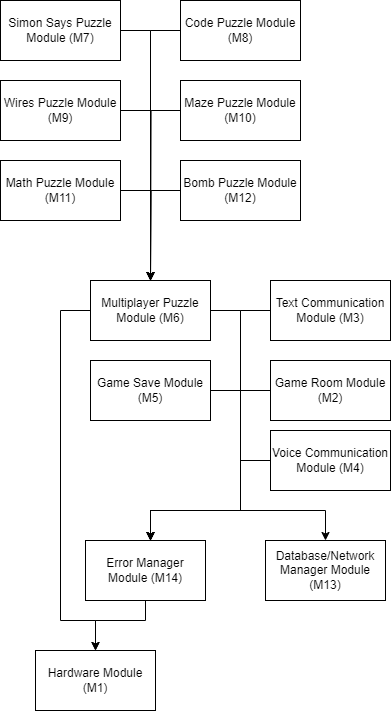
\includegraphics[width=0.7\textwidth]{Capstone/docs/SoftArchitecture/ModuleHierarchy.png}
\caption{Use hierarchy among modules}
\label{FigUH}
\end{figure}

%\section*{References}
\section{User Interfaces}
Here are some photos showing the user interface design of the application:

\begin{figure}[H]
\centering
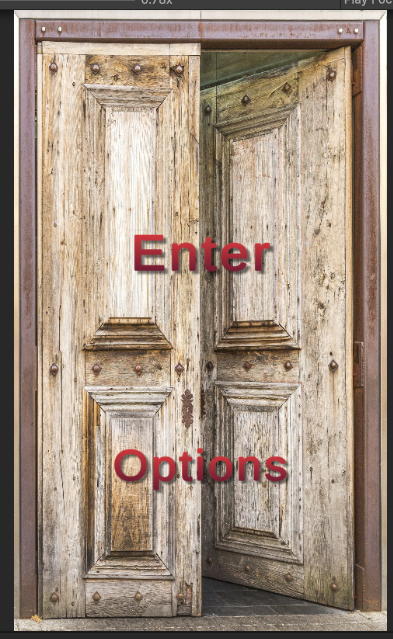
\includegraphics[width=0.3\textwidth]{Capstone/docs/SoftArchitecture/MainMenu.png}
\caption{Main Menu Screen}
\label{FigUH}
\end{figure}

\begin{figure}[H]
\centering
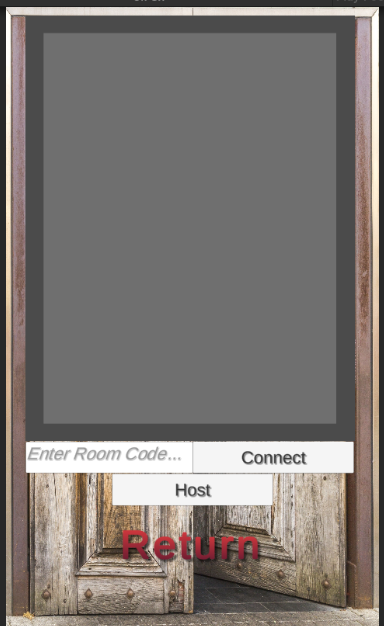
\includegraphics[width=0.3\textwidth]{Capstone/docs/SoftArchitecture/HostScreen.png}
\caption{Host/Join Game Screen}
\label{FigUH}
\end{figure}

\begin{figure}[H]
\centering
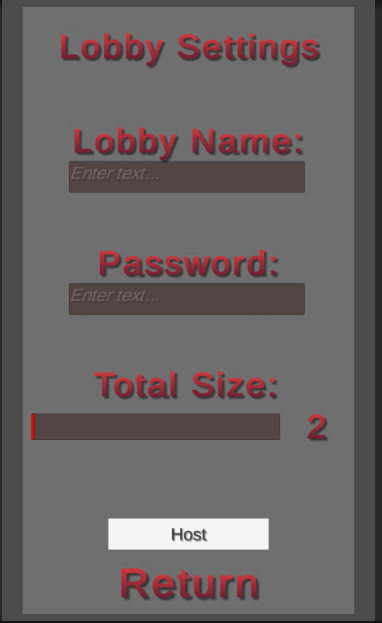
\includegraphics[width=0.3\textwidth]{Capstone/docs/SoftArchitecture/CreateLobbyScreen.png}
\caption{Create Lobby Screen}
\label{FigUH}
\end{figure}


\begin{figure}[H]
\centering
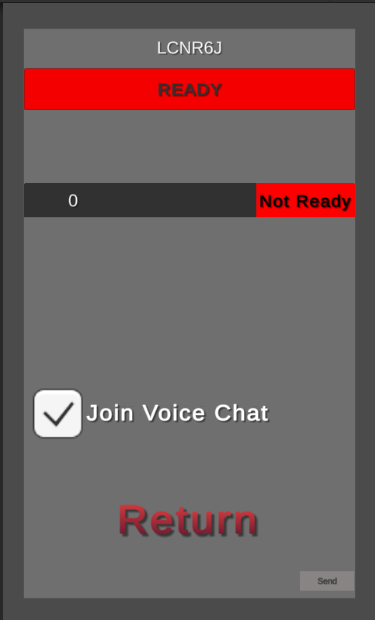
\includegraphics[width=0.3\textwidth]{Capstone/docs/SoftArchitecture/LobbyScreen.png}
\caption{Lobby Screen}
\label{FigUH}
\end{figure}


\begin{figure}[H]
\centering
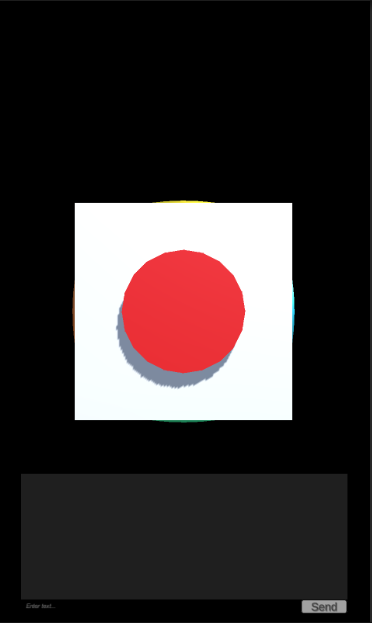
\includegraphics[width=0.3\textwidth]{Capstone/docs/SoftArchitecture/InGameScreen.png}
\caption{In Game Screen}
\label{FigUH}
\end{figure}


\section{Timeline} \label{Rev0Timeline}
The following timeline describes the work that needs to be completed in order for the implementation of Rev 0 to be complete

\begin{itemize}
    \item Jan 15 - Jan 25:  Completion of Game Room Module, Text Communication Module, Voice Communication Module, Database/Network Manager Module
    \begin{itemize}
        \item     Matthew will work on the completion of the Game Room Module. Ethan and Kieran will work on the completion of the Text and Voice Communication Modules.
    \end{itemize}
    \item Jan 20 - Feb 6: Completion of Game Save Module, Multiplayer Puzzle Module, Simon Says Puzzle Module, Code Puzzle Module, Wires Puzzle Module, Maze Puzzle Module, Math Puzzle Module, Bomb Puzzle Module
    \begin{itemize}
        \item Sam will work on the completion of the Game Save Module. Matthew will work on the completion of the Multiplayer Puzzle Module, and the Maze Puzzle Module. Ethan will work on the completion of the Simon Says Puzzle Module. Kieran will work on the completion of the Bomb Puzzle Module. Sam will work on the completion of the Math Puzzle and the Wires Puzzle Module.
    \end{itemize}
    \item Jan 28 - Feb 10: Completion of Error Manager Module, Database/Network Manager Module, and Testing and Verification
    \begin{itemize}
        \item Kieran and Matthew will work on the completion of the Error Manager Module. Ethan and Sam will work on the completion of the Database/Network Manager Module. All group members will work on completing the testing and verification required to make sure application is ready for Revision 0.
    \end{itemize}

\end{itemize}

\bibliographystyle {plainnat}
\bibliography{References}

\newpage{}

\end{document}